\begin{figure}
	\tikzsetnextfilename{versore-tangente-normale}
	\centering
	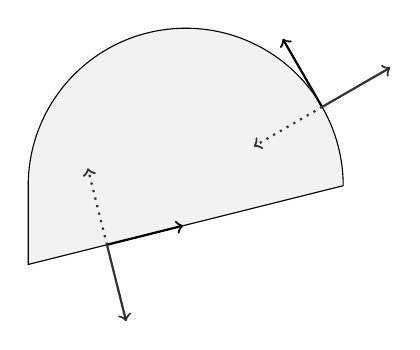
\begin{tikzpicture}
		\draw[fill=black!5!white] (-2,0) -- (-2,-1) -- (2,0) arc (0:180:2);
		% Considero la curva orientata in senso antiorario

		% L'arco è parametrizzato da f(t)=(2*cos(t), 2*sin(t)), t in [0,pi]
		\coordinate (t1) at (1.732,1); % t=pi/6
		\draw[->,thick,black] (t1) -- ++(-.5,.866); % Versore tangente
		\draw[->,thick,black!80!white] (t1) -- ++(.866,.5); % Versore normale uscente
		\draw[->,thick,black!80!white,dotted] (t1) -- ++(-.866,-.5); % Versore normale entrante

		% La retta in basso è parametrizzata da f(t)=(-2+4*t, -1+t), t in [0,1]
		\coordinate (t2) at (-1,-.75); % t=1/4
		\draw[->,thick,black] (t2) -- ++(0.97,.243); % Versore tangente
		\draw[->,thick,black!80!white] (t2) -- ++(.243,.-0.97); % Versore normale uscente
		\draw[->,thick,black!80!white,dotted] (t2) -- ++(-.243,0.97); % Versore normale entrante
	\end{tikzpicture}
	\caption{I versori tangenti e normali al bordo di un dominio regolare di $\R^2$.
		Tale bordo è orientato in senso positivo se è percorso in senso antiorario: in questo modo il versore normale (con tratto continuo) è uscente, e il versore tangente è come indicato.
	L'orientazione in senso negativo dà invece il versore normale entrante (con tratto punteggiato) e il versore tangente opposto.}
	\label{fig:versore-tangente-normale}
\end{figure}
